\documentclass[11pt]{article}
\usepackage{fullpage}
\usepackage{graphics,epsfig,color}
\usepackage{wrapfig}
\usepackage{times}
\usepackage{setspace}
\usepackage{amsmath,amsthm,amssymb}
\usepackage{url}
\usepackage{fancyhdr}
\usepackage{enumitem}
\pagestyle{fancy}


\newtheorem{theorem}{Theorem}[section]
\newtheorem{corollary}{Corollary}[section]
\newtheorem{lemma}{Lemma}[section]
\newtheorem{problem}{Problem}
\newtheorem{definition}{Definition}[section]
\newtheorem{observation}{Observation}[section]
\newtheorem{example}{Example}[section]
\newtheorem{openproblem}{Open Problem}[section]
\newtheorem{fact}{Fact}[section]

\newcommand{\qedsymb}{\hfill{\rule{2mm}{2mm}}}
\newenvironment{proofsketch}
{
	\begin{trivlist}
	\item[\hspace{\labelsep}{\noindent Proof Sketch: }]
}{\qedsymb\end{trivlist}}



%the following few lines until usepackage{algorithm2e} is to avoid the
%conflicts of algorithm2e with other packages.
\makeatletter
\newif\if@restonecol
\makeatother
\let\algorithm\relax
\let\endalgorithm\relax
\usepackage[ruled,vlined,linesnumbered]{algorithm2e}

\newcommand{\remove}[1]{}



%--------------------------------


\begin{document}

	\renewcommand{\headrulewidth}{0.4pt}
	\setlength{\headheight}{38.0pt}
	\fancyhead[L]{\bf CSCD359 Homework 4, Winter 2012, 
	Eastern Washington University. Cheney, Washington. \\
	\bigskip Name: Eric Fode\hspace{40mm}EWU ID:00530214}


	\noindent{\bf Solution for Problem 1}\\
		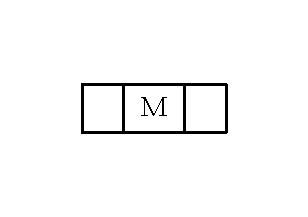
\includegraphics[scale=.5]{step1.pdf}
		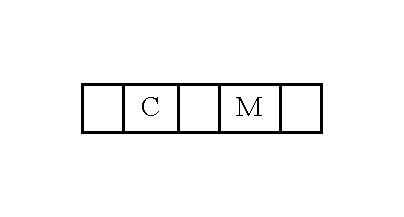
\includegraphics[scale=.5]{step2.pdf}
		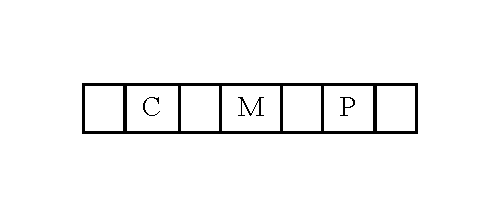
\includegraphics[scale=.5]{step3.pdf}
		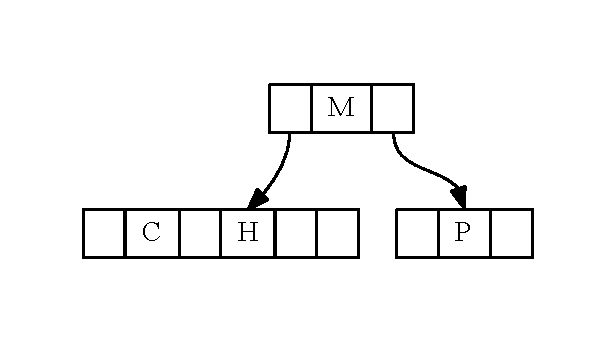
\includegraphics[scale=.5]{step4.pdf}\\
		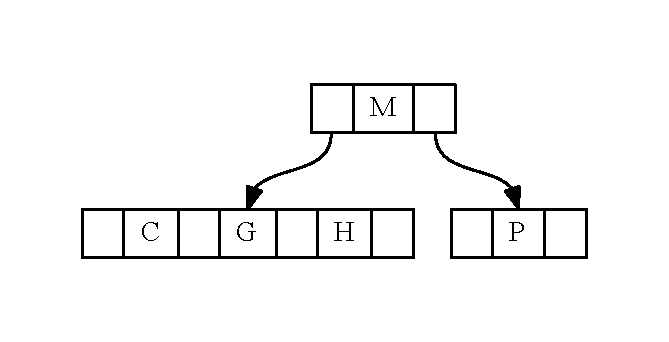
\includegraphics[scale=.5]{step5.pdf}
		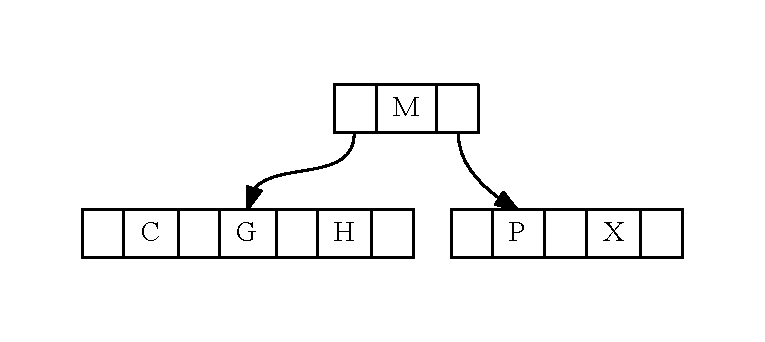
\includegraphics[scale=.5]{step6.pdf}\\
		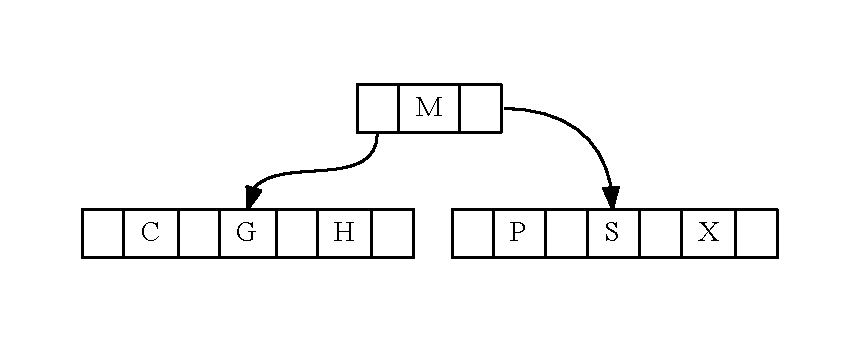
\includegraphics[scale=.5]{step7.pdf}
		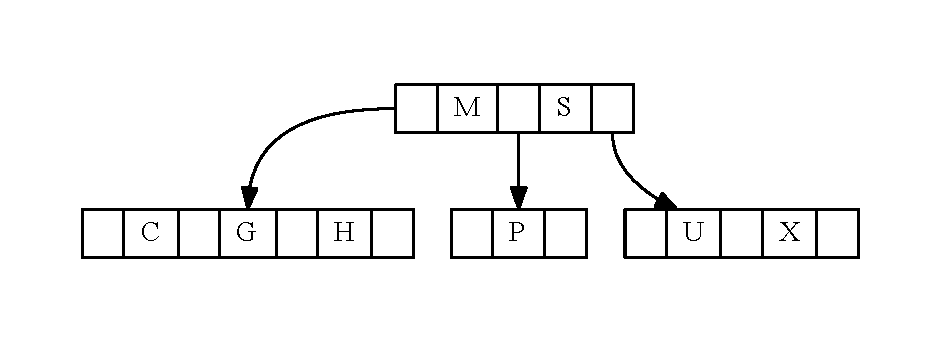
\includegraphics[scale=.5]{step8.pdf}\\
		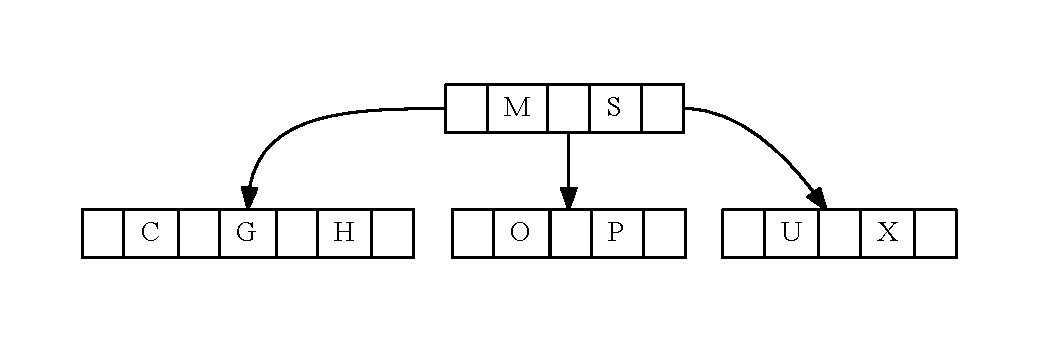
\includegraphics[scale=.5]{step9.pdf}\\
		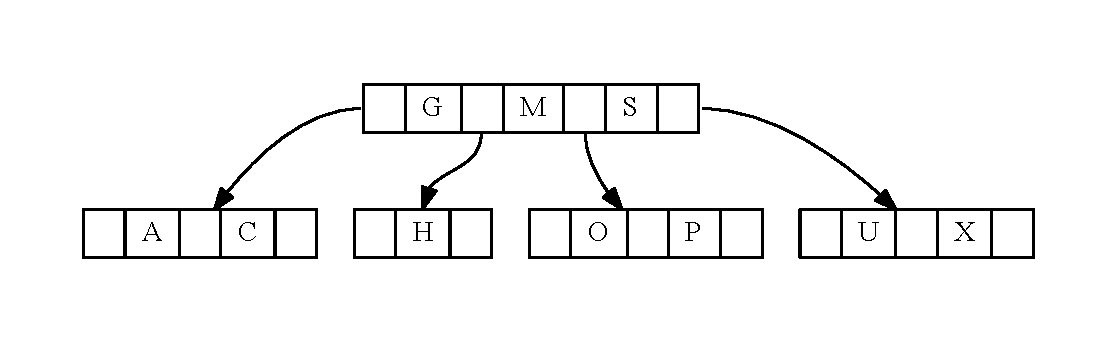
\includegraphics[scale=.5]{step10.pdf}\\
		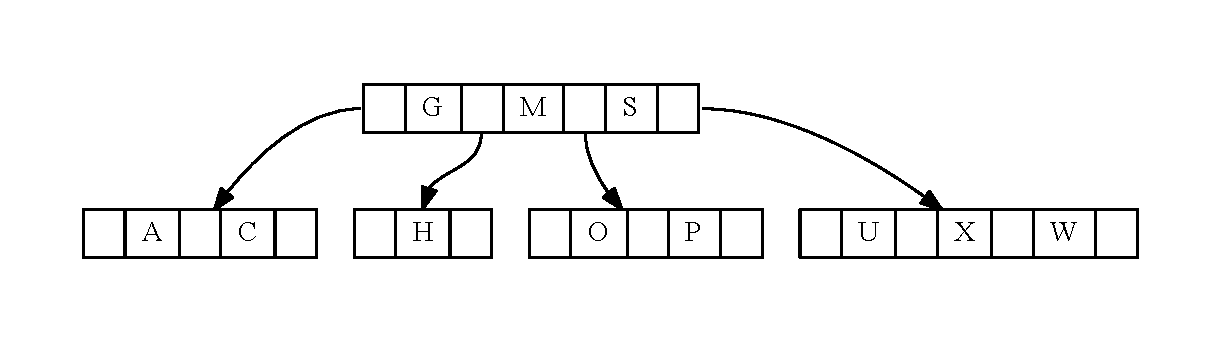
\includegraphics[scale=.5]{step11.pdf}\\	
		
	\newpage
	
	\noindent{\bf Solution for Problem 2}\\
		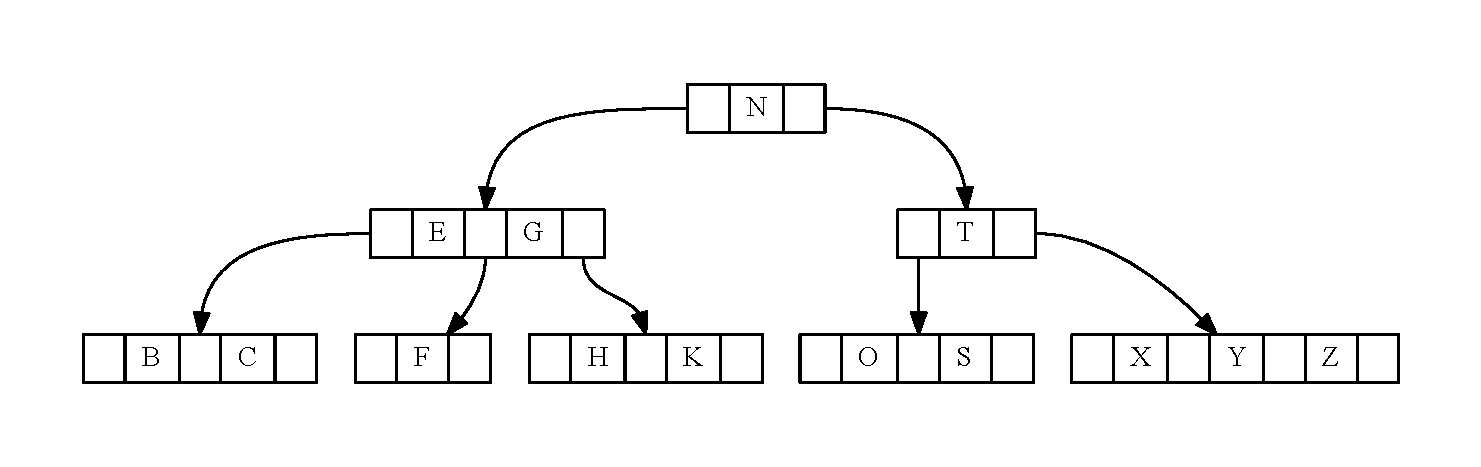
\includegraphics[scale=.5]{bstep1.pdf}\\
		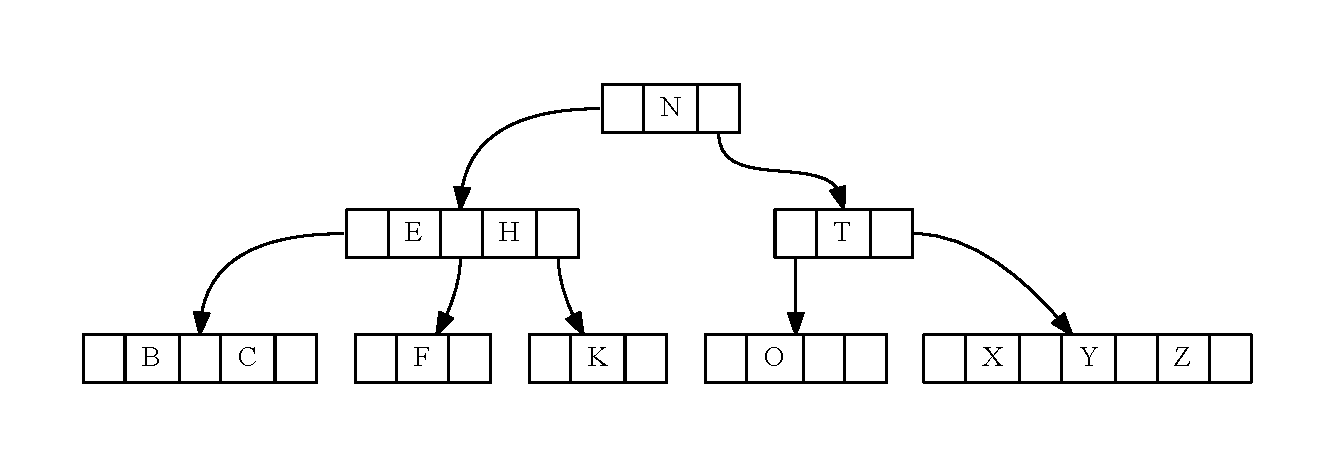
\includegraphics[scale=.5]{bstep2.pdf}\\
		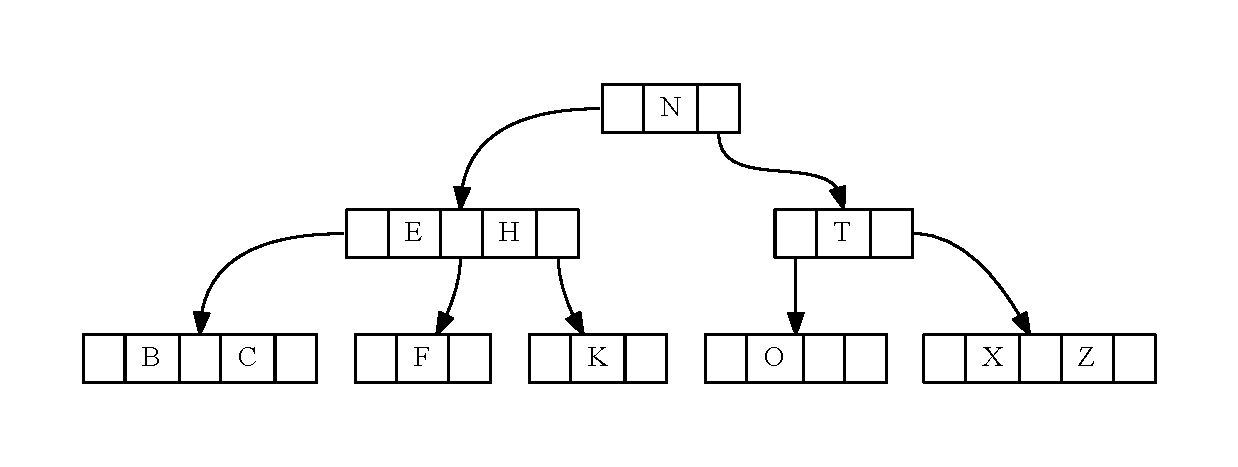
\includegraphics[scale=.5]{bstep3.pdf}\\
		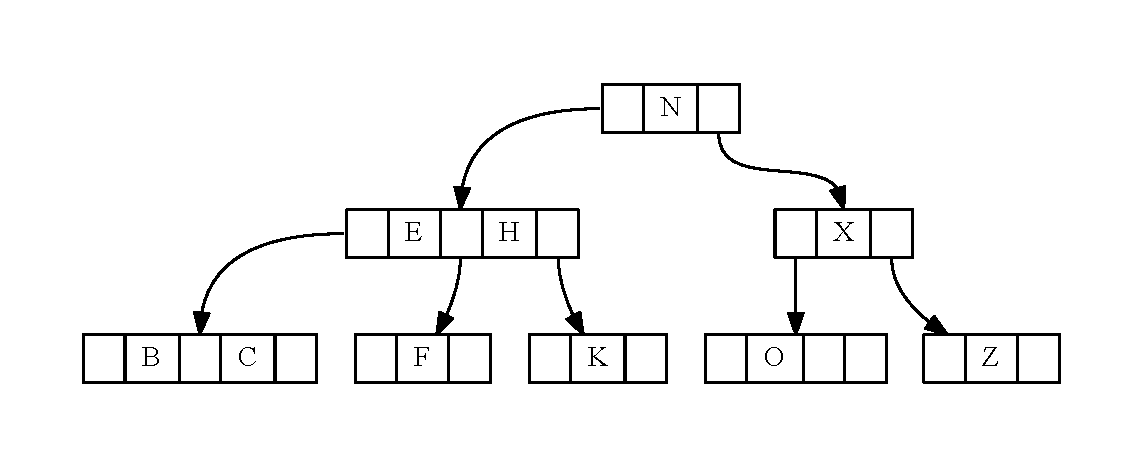
\includegraphics[scale=.5]{bstep4.pdf}\\
		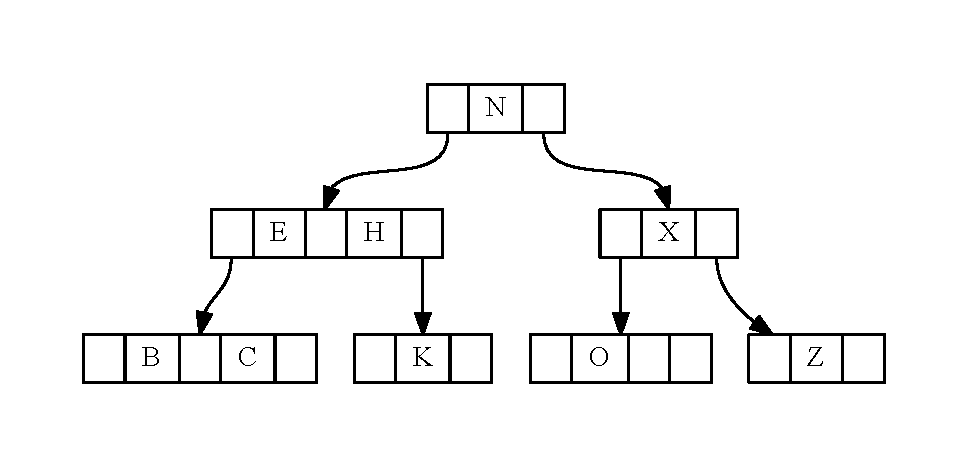
\includegraphics[scale=.5]{bstep5.pdf}\\
		
	\newpage
	\noindent{\bf Solution for Problem 3}\\
	
	\noindent{\bf Part 1 Idea:} To find the max of a tree given the root of the tree simply navigate right and down until there are no more nodes to iterate through
	
	\noindent{\bf Part 1 Algorithm:}\\
	\begin{algorithm}[H]
		\NoCaptionOfAlgo
		\caption{\bf bTreeFindMax($root$)}
		\SetKwData{ChildMax}{childMax}\SetKwData{Null}{null}
		\SetKwFunction{BTreeFindMax}{bTreeFindMax}
		\SetKwFunction{DISKREAD}{DISKREAD}
		\KwIn{The root of a b-tree that is in memory}
		\KwResult{The max item in the b-tree}
		
		\Begin{
			\If{$root == null$}
			{
				\Return $null$;
			}
			\ChildMax $\leftarrow$ \BTreeFindMax{\DISKREAD{$root.lastChild$}}\;
		
			\If{\ChildMax $== null$}
			{
				\Return{$root$, $root[root.n-1]$}\;
			}	
			\Else
			{
				\Return{\ChildMax}\;
			}
		}
	\end{algorithm}
	
	\noindent{\bf Part 1 Analysis:} This should take $O(log(h))$ time including disk operations
	\bigskip
	

	\noindent{\bf Part 2 Idea:} To find the predecessor of a node if the index of the key is 0 go to the parent and return the last key that less then the first key. If index greater then 0 check for a child nodes attached to the i'th slot for a child node (the position directly left of i)  less then i if one exists the predecessor is the max of the b-tree rooted at the roots child, if no child exists then the predecessor is the key at $i-1$.
	\newpage
	\noindent{\bf Part 2 Algorithm:}\\
	\begin{algorithm}[H]
		\NoCaptionOfAlgo
		\caption{\bf BTreePredecessor($node$, $i$)}
		\SetKwFunction{BTreeFindMax}{BTreeFindMax}
		\SetKwFunction{DISKREAD}{DISKREAD}
		\SetKwFunction{Continue}{continue}
		\KwIn{A node and it's i'th key}
		\KwResult{$predecessorNode$, $j$ where "predecessorNode" is the node that contain the predecessor key which is at position j }
		\Begin{
			\If{$parent.exsists == falsei == 0$ }
			{
				\Return{$null$}\;
			}
			\If{$i > 0$}
			{
				\If{$root.child(i).exists()$}
				{
					\Return{ \BTreeFindMax{\DISKREAD{$root.child(i)$}}}\;
				}
				\Else
				{
					\Return{$root, i-1$}
				}
			}
			\If{$i == 0$}
			{
				$curNode \leftarrow root$\;
				\While{$true$}
				{
					$curNode \leftarrow$ \DISKREAD{$curNode.parent$}\;
					\For{$index \leftarrow 0;root[i] > curNode[index]$ {\bf and} $index < curNode.n;index++$}{}
					\If{$root[i] > curNode[index]$}
					{
						$continue$\;
					}
					\Else
					{
						\Return{$curNode,index$}\;
					}
				}
			}
		}
	\end{algorithm}
	\noindent{\bf Part 2 Analysis:} This should take $O(log(h)t)$ time
	\bigskip
	
	\noindent{\bf Solution for Problem 4}\\
	Find the number of items that can fit into memory, load that much of the array into memory, Sort it. Continue loading contiguous pieces of the array into memory and sorting them. After the whole array has been pass through begin a series of merge passes. for $i = numberOfParts$ iterate through contiguous parts of the array merging them together one chunk at a time repeat this process until $i=1$. At this point the array will be sorted.
	
\end{document}